\documentclass[journal]{IEEEtran}

\usepackage{cite}
\usepackage{amsmath,amssymb,amsfonts}
\usepackage{amsthm}
\newtheorem{definition}{Definition}
\newtheorem{proposition}{Proposition}
\usepackage{graphicx}
\usepackage{textcomp}
\usepackage{xcolor}
\usepackage{booktabs}
\usepackage{multirow}
\usepackage{array}
\usepackage{url}
\usepackage{hyperref}
\usepackage{siunitx}
\usepackage{pgfplots}
\pgfplotsset{compat=1.17}
\usepackage{tikz}
\usetikzlibrary{shapes,arrows,positioning,calc,matrix}
\usepackage{placeins}
\usepackage{float}
\usepackage{dblfloatfix}
\usepackage{caption}
\usepackage{colortbl}
\usepackage{microtype}

% ---- siunitx: decimal alignment ----
\sisetup{
  detect-weight,
  detect-family,
  table-align-text-pre  = false,
  table-align-text-post = false,
  group-digits          = false
}

% ---- table caption ----
\captionsetup{font=small,labelfont=bf,labelsep=period,skip=4pt}
\captionsetup[table]{position=top}
\captionsetup[figure]{position=bottom}

% ---- table global parameters ----
\setlength{\tabcolsep}{4pt}
\renewcommand{\arraystretch}{1.18}

% ---- zebra definitions retained but NOT used (clean booktabs) ----
\definecolor{zebra}{HTML}{F4F4F4}
\definecolor{grouphead}{HTML}{E8ECF1}
\newcommand{\zebrarow}{\rowcolor{zebra}}

\begin{document}

\title{Protocol-Aware Robust Evaluation of Rating-Prediction Recommenders: Functional Collapse Under Cold-Start Splits}

\author{
\IEEEauthorblockN{Anonymous Authors}
\IEEEauthorblockA{Under Review}
}

\maketitle

\begin{abstract}
Offline evaluation protocols are often treated as secondary experimental settings in recommender-system research. However, different protocols determine which user- or item-specific signals are available during evaluation, and may therefore alter the effective model being assessed. This study investigates this issue through a multi-seed empirical evaluation of 12 rating-prediction recommenders from four model families (Bias, Matrix Factorization, Deep, and Adaptive) across three public datasets (ML-1M, GoodBooks, Book-Crossing) and three evaluation protocols: strict cold-start (SC), warm-random (WR), and warm-temporal (WT) splitting. Across 288 runs (12 models $\times$ 8 dataset--protocol combinations $\times$ 3 seeds), we observe protocol-induced functional collapse: under SC, UserBias degenerates exactly into GlobalMean ($\Delta$RMSE~$=0.00000$ on all datasets) because user-specific parameters are unestimable for unseen test users, and UserItemBias collapses toward ItemBias. We further show that model rankings are highly protocol-dependent, with rank shifts of up to 10 positions and inter-protocol Kendall $\tau$ approaching zero (GoodBooks SC-vs-WT $= -0.030$). To characterize this behavior, we introduce a protocol-robustness diagnostic suite consisting of the Protocol Sensitivity Index (PSI), inter-protocol Kendall $\tau$, and Protocol Regret. The results suggest that recommender evaluation should report multi-protocol robustness rather than relying on a single offline split, especially when deployment scenarios involve cold-start users or temporal drift.
\end{abstract}

\begin{IEEEkeywords}
Recommender systems, evaluation methodology, offline evaluation, cold-start, protocol sensitivity, model robustness, protocol-aware model selection, deployment risk
\end{IEEEkeywords}

% ============================================================================
% 1. INTRODUCTION
% ============================================================================
\section{Introduction}
\label{sec:intro}

Recommendation systems are fundamental to modern information access, yet their offline evaluation remains surprisingly sensitive to methodological choices that are often treated as secondary. A common assumption in the literature is that model quality is determined by architecture, and that a model judged superior under one offline protocol will remain superior when deployed. This paper shows that the choice of evaluation protocol does not merely change test difficulty; it changes the functional form of the evaluated recommender, because different protocols determine which user- or item-specific signals are estimable at test time.

We investigate how three widely-used evaluation protocols affect model rankings, each commonly used as a proxy for a recognizable deployment scenario:
\begin{itemize}
    \item \textbf{Strict cold-start (SC)}: test users never appear in the training set---commonly used as a proxy for \emph{new-user onboarding}, where the system must serve users with no interaction history;
    \item \textbf{Warm-random (WR)}: random row-level splitting where the same user can appear across train/test---commonly used as a proxy for \emph{continued recommendation for existing users} and as an offline approximation of A/B-test comparisons;
    \item \textbf{Warm-temporal (WT)}: time-ordered splitting where training strictly precedes testing---commonly used as a proxy for \emph{time-drifted environments}, where the system is evaluated on future behavior that may have shifted.
\end{itemize}

Although the unavailability of user-specific parameters under cold-start may appear intuitive, its empirical consequence is rarely quantified as a change in the effective model being evaluated. Across three datasets spanning a $3000\times$ density range and 12 models from four architectural families, we observe that protocol selection does more than perturb rankings---it changes which model components are functionally usable. Most strikingly, under strict cold-start the UserBias model collapses \emph{exactly} onto GlobalMean (RMSE difference~$=0.00000$ on all three datasets), because test users are unseen and user-specific biases cannot be estimated. This is a mechanism-level change in the effective model, not merely a ranking fluctuation: a practitioner who deploys UserBias under cold-start conditions is, in effect, deploying GlobalMean.

The main contributions of this work are as follows. First, we provide a controlled multi-seed evaluation of 12 rating-prediction recommenders across three datasets and three offline evaluation protocols (288 runs), showing that protocol choice systematically changes model rankings. Second, we identify and formalize \emph{protocol-induced functional collapse}, a mechanism by which protocol-dependent data availability disables model components such as user-specific bias terms, and which generalizes to any model relying on per-user parameters that cannot transfer to cold test users. Third, we quantify model-family $\times$ protocol interactions, showing that cold-start, random, and temporal protocols favor different structural signals (item-side priors vs.\ static collaboration vs.\ behavioral/adaptive fusion). Fourth, we introduce a protocol-robustness diagnostic suite based on the Protocol Sensitivity Index (PSI), inter-protocol Kendall $\tau$, and Protocol Regret to support deployment-aware model selection.

% ============================================================================
% 2. RELATED WORK
% ============================================================================
\section{Related Work}
\label{sec:related}

\subsection{Recommender Evaluation and Benchmark Instability}
A growing body of work has questioned whether complex neural models reliably outperform simpler baselines and whether benchmark conclusions are stable. Dacrema et al.~\cite{dacrema2019we,dacrema2021troubling} showed that many neural recommendation methods do not significantly outperform simple baselines when hyperparameters are properly tuned, and Ca{\~n}amares and Castells~\cite{canamares2018should} similarly found that strong popularity-based baselines are difficult to beat under common evaluation regimes. Standard accuracy metrics for recommendation have been surveyed by Gunawardana and Shani~\cite{gunawardana2009survey}, and unified evaluation frameworks such as RecBole~\cite{zhao2021recbole} have been developed to facilitate reproducible comparison. These works primarily focus on metric choice, hyperparameter fairness, and baseline strength; the present study complements them by treating the \emph{splitting protocol} itself as a factor that can alter the effective model.

\subsection{Cold-Start and Protocol-Dependent Data Availability}
Cold-start recommendation has been addressed through content-based methods~\cite{schein2002methods}, meta-learning approaches~\cite{vartak2017meta}, and hybrid architectures that fuse collaborative and content signals~\cite{elkahky2015multi}. The boundary between cold and warm users is inherently protocol-dependent: under strict user-level splitting, all test users are unseen; under row-level random splitting, the same user can appear in both training and test sets; under temporal splitting, the system is evaluated on future behavior. Although these protocols are well established, their impact on which model components remain estimable---and consequently on model rankings---has received limited systematic study.

\subsection{Robust Model Comparison and Reproducibility}
Matrix factorization~\cite{koren2009matrix} and its learning-to-rank extensions such as BPR~\cite{rendle2009bpr} form the classical collaborative-filtering backbone, while embarrassingly shallow autoencoders~\cite{steck2019ease} have shown that simple linear models can be competitive on sparse data. On the neural side, NeuMF~\cite{he2017neural}, DeepFM~\cite{guo2017deepfm}, and industrial-scale deep models~\cite{covington2016deep} represent the higher-complexity end, complemented by sequential approaches~\cite{kang2018sasrec,sun2019bert4rec} and graph neural networks~\cite{wang2019ngcf,he2020lightgcn}. Multi-seed evaluation and reproducibility-friendly frameworks have become standard practice in this line. However, existing studies have examined cold-start recommendation, benchmark reproducibility, and model comparison, but less attention has been paid to how evaluation protocols change the set of estimable model components. This work addresses this gap by treating the protocol as a factor that can alter the effective recommender being evaluated, and by providing protocol-robustness diagnostics that go beyond single-protocol point estimates.

% ============================================================================
% 3. METHODOLOGY
% ============================================================================
\section{Methodology}
\label{sec:method}

\subsection{Datasets}
\label{sec:datasets}

We evaluate on three public datasets spanning a $3000\times$ density range:

\begin{table}[!t]
\centering
\caption{Dataset statistics.}
\label{tab:datasets}
\footnotesize
\begin{tabular}{@{}lrrrcc@{}}
\toprule
Dataset & Users & Items & Ratings & Density & Timestamps \\
\midrule
ML-1M & 6,040 & 3,706 & 1,000,209 & 4.47\% & Yes \\
GoodBooks & 53,424 & 13,667 & 5,342,431 & 0.73\% & Yes \\
Book-Crossing & 278,858 & 271,379 & 1,149,780 & 0.0015\% & No \\
\bottomrule
\end{tabular}
\end{table}

ML-1M is a dense movie rating dataset with real timestamps. GoodBooks is a moderately sparse book rating dataset. Book-Crossing is extremely sparse, with a density three orders of magnitude lower than ML-1M. Since Book-Crossing lacks timestamps, only strict cold-start and warm-random protocols are evaluated on this dataset, giving eight valid dataset--protocol combinations.

\subsection{Evaluation Protocols}
\label{sec:protocols}

We define three evaluation protocols that represent common practice in the literature:

\begin{table}[!t]
\centering
\caption{Evaluation protocol definitions.}
\label{tab:protocols}
\footnotesize
\begin{tabular}{@{}lll@{}}
\toprule
Protocol & Split method & Training-set users/items \\
\midrule
Strict Cold (SC) & User-level & Test users never in train \\
Warm-Random (WR) & Row-level random & Same user can cross sets \\
Warm-Temporal (WT) & Time-ordered & Train $<$ Val $<$ Test \\
\bottomrule
\end{tabular}
\end{table}

\subsection{Compared Models}
\label{sec:models}

We evaluate 12 models from four architectural families, ordered by increasing complexity (levels 1--4):

\begin{table}[!t]
\centering
\caption{Compared models and complexity levels.}
\label{tab:models}
\footnotesize
\begin{tabular}{@{}llcl@{}}
\toprule
Model & Category & Complexity & Description \\
\midrule
GlobalMean & Bias & 1 & Global rating average \\
UserBias & Bias & 1 & User-specific bias \\
ItemBias & Bias & 1 & Item-specific bias \\
UserItemBias & Bias & 1 & User + Item bias \\
SVD & MF & 2 & Matrix factorization \\
NeuMF & Deep & 3 & Neural collaborative filtering \\
DeepFM & Deep & 3 & FM + Deep network \\
BehaviorMLP & Deep & 3 & Behavior feature MLP \\
ProfileMLP & Deep & 3 & Profile feature MLP \\
Hybrid & Deep & 3 & Profile + Behavior fusion \\
DualHard & Adaptive & 4 & Hard cold/warm switch \\
DualSoft & Adaptive & 4 & Learned soft gating \\
\bottomrule
\end{tabular}
\end{table}

All models are implemented within a unified framework with consistent data loading, preprocessing, and evaluation pipelines.

\textbf{Feature construction and leakage control.} The Bias and MF families use only user/item identifiers and observed ratings. The deep models use two auxiliary feature groups: (i) \emph{profile features} (user demographics and item metadata available at training time, e.g., user age and item genre) and (ii) \emph{behavioral features} (training-set interaction statistics such as per-user mean rating, rating count, and per-item popularity). To prevent leakage, all auxiliary features are computed \emph{strictly from the training split}: profile and behavioral statistics for any test user are derived only from that user's training-set presence. Under SC, where a test user has no training history, behavioral features for that user are unavailable and fall back to the global training-set average, so the behavioral signal is effectively reset to a constant; this is consistent with the cold-start setting and does not introduce future information. ProfileMLP uses only profile features, BehaviorMLP uses only behavioral features, Hybrid fuses both via concatenation, and the Dual models route between a cold-path (profile/global-statistic) and a warm-path (behavioral/MF) predictor.

\begin{figure*}[!t]
\centering
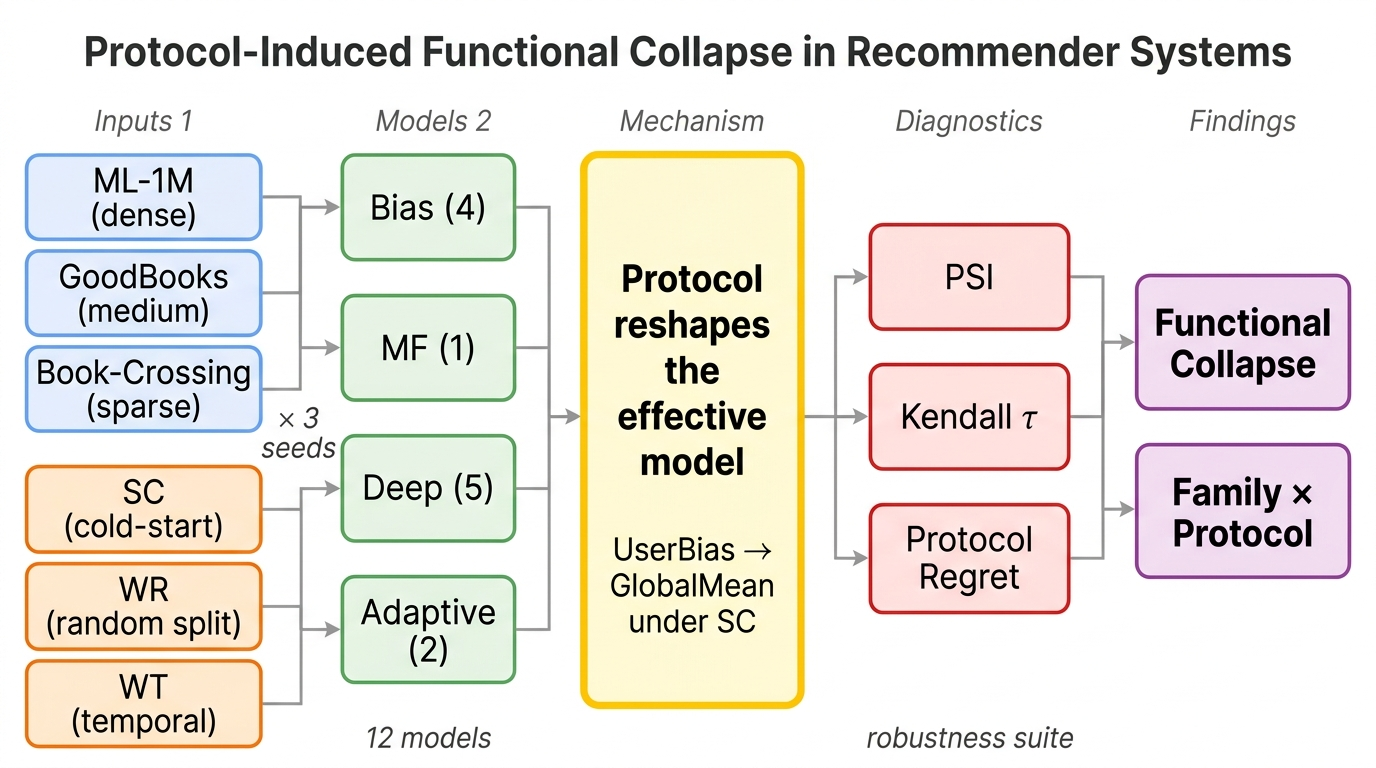
\includegraphics[width=0.85\textwidth]{figures/机制图.png}
\caption{Research framework. Three datasets span a $3000\times$ density range; three protocols (SC/WR/WT) and three seeds yield 288 runs across 12 models from four families. The protocol reshapes the \emph{effective} model (e.g., UserBias degenerates to GlobalMean under SC); multi-seed evaluation exposes protocol-induced functional collapse and family $\times$ protocol interaction through the PSI, Kendall $\tau$, and Protocol Regret diagnostics.}
\label{fig:framework}
\end{figure*}

\subsection{Formal Definition of Protocol-Induced Functional Collapse}
\label{sec:formal_collapse}

To make the core phenomenon precise rather than purely observational, we formalize it as a property of the estimable parameter set under a given protocol. Consider a general rating-prediction model with prediction function
\begin{equation}
\hat{r}_{ui} = \mu + b_u + b_i + f(u, i),
\label{eq:general}
\end{equation}
where $\mu$ is the global mean, $b_u$ and $b_i$ are user- and item-specific terms, and $f(u,i)$ is an optional interaction term (e.g., MF inner product or a neural function). Let $U_{\text{train}}$ and $I_{\text{train}}$ denote the sets of users and items observed in the training split, and let $\Theta_{\text{est}}(p)$ denote the set of model parameters that are estimable from training data under protocol $p$.

\begin{definition}[Functional Collapse]
A model $M$ with nominal parameter set $\Theta$ undergoes \emph{protocol-induced functional collapse} under protocol $p$ if $\Theta_{\text{est}}(p) \subsetneq \Theta$, i.e., the protocol renders a subset of parameters unestimable, and the model's prediction function reduces to that of a simpler submodel $M'$ with $\Theta' = \Theta_{\text{est}}(p)$.
\end{definition}

\begin{proposition}[Collapse of UserBias under Strict Cold-Start]\label{prop:collapse}
Under strict cold-start (SC), every test user $u \in U_{\text{test}}$ satisfies $u \notin U_{\text{train}}$, so $b_u$ has no training signal. If the system adopts the standard fallback $b_u = 0$ for unseen users, the UserBias prediction $\hat{r}_{ui} = \mu + b_u$ reduces to $\hat{r}_{ui} = \mu$, which is prediction-equivalent to GlobalMean. Similarly, UserItemBias reduces to ItemBias, with any residual gap attributable to regularization or numerical effects rather than to a user-side signal.
\end{proposition}

This formulation reframes the phenomenon as a property of the estimable parameter set: the protocol does not merely change test difficulty, it changes the active parameterization of the evaluated model. We use the term \emph{functional collapse} to denote this protocol-dependent reduction in the active parameterization of a recommender, such that a nominally richer model becomes prediction-equivalent or near-equivalent to a simpler submodel. The mechanism generalizes beyond UserBias to any model component whose parameters depend on entities (users, items, or interactions) that are absent from the training split.

\subsection{Evaluation Metrics}
\label{sec:metrics}

Since the task is formulated as rating prediction, we use RMSE as the primary evaluation metric. We additionally define three protocol-robustness diagnostics that summarize behavior \emph{across} protocols.

\subsection{Protocol Sensitivity Index (PSI)}
\label{sec:psi}

To quantify how sensitive a model's ranking is to protocol choice, we define the Protocol Sensitivity Index:
\begin{equation}
PSI_m = \max_{p}(Rank_{m,p}) - \min_{p}(Rank_{m,p})
\label{eq:psi}
\end{equation}
where $Rank_{m,p}$ denotes the rank of model $m$ under protocol $p$. A higher PSI indicates greater protocol sensitivity. For Book-Crossing, which has only two protocols, PSI is computed over strict cold-start and warm-random.

\subsection{Bias-Normalized RMSE (BNR)}
\label{sec:bnr_def}

To assess whether a model improves over simple bias baselines, we define the Bias-Normalized RMSE:
\begin{equation}
BNR_m = \frac{RMSE_m}{RMSE_{best\_bias}}
\label{eq:bnr}
\end{equation}
where $RMSE_{best\_bias}$ is the RMSE of the best-performing bias baseline under the same dataset and protocol. $BNR=1.0$ denotes parity with the best bias baseline; $BNR<1.0$ denotes an improvement.

\subsection{Inter-Protocol Kendall Tau}
\label{sec:kendall_def}

To measure ranking consistency between two protocols on the same dataset, we compute Kendall's $\tau$ over the 12 model ranks. $\tau=+1$ indicates identical rankings, $\tau=0$ uncorrelated rankings, and $\tau=-1$ fully reversed rankings. Low or near-zero $\tau$ between two protocols signals that they effectively select different models.

\subsection{Protocol Regret}
\label{sec:regret_def}

To distinguish models that are robust across protocols from those that excel only under specific protocols, we define per-protocol regret:
\begin{equation}
Regret_{m,d,p} = RMSE_{m,d,p} - RMSE_{best,d,p}
\label{eq:regret}
\end{equation}
where $RMSE_{best,d,p}$ is the lowest RMSE achieved by any model on dataset $d$ under protocol $p$. We then summarize each model by its \emph{mean regret} (averaged over available protocols) and its \emph{worst regret} (the maximum per-protocol regret). Low mean and low worst regret indicate robust models; low mean with high worst regret indicates protocol-specialized models.

\subsection{Experimental Setup}
\label{sec:setup}

All experiments are repeated over three random seeds (2024, 2025, 2026). Each seed controls both model initialization and the randomized split draw (row-level shuffling for WR, user-level partition for SC, and timestamp cut-point for WT within the fixed 80/10/10 ratio), so seed variation captures both initialization noise and split-draw noise. We evaluate 12 models across eight valid dataset--protocol combinations: three protocols for ML-1M, three for GoodBooks, and two for Book-Crossing. The final evaluation therefore consists of $12 \times 8 \times 3 = 288$ model--protocol--seed runs. All reported RMSE values are the mean over the three seeds, with standard deviations shown in parentheses. We focus on effect sizes (mean $\pm$ std, rank shifts, Kendall $\tau$, regret) rather than $p$-values; the rank-level findings (PSI, Kendall $\tau$, Protocol Regret) are discrete and stable across the three seeds, so we report them as point estimates rather than with bootstrap intervals.

\textbf{Data preprocessing.} All three datasets use the same preprocessing pipeline: ratings are retained as raw explicit scores, users and items with fewer than a minimal activity threshold (5 interactions) are filtered, and global rating statistics are recomputed per split to prevent leakage. For ML-1M and GoodBooks, timestamps are used only by the WT protocol; for Book-Crossing, which lacks timestamps, only SC and WR are evaluated.

\textbf{Split ratios.} For each dataset--protocol combination we use a fixed 80\%/10\%/10\% train/validation/test split. Under SC the split is at the user level (disjoint test users); under WR it is a row-level random split (the same user may appear in train and test); under WT the split is time-ordered, with the training window strictly preceding validation, which strictly precedes testing.

\textbf{Split statistics and item cold-start handling.} Under SC, all test users are by construction absent from the training set (100\% user cold-start), while test items are retained only if they also appear in training; any test rating on an item unseen in training is dropped from evaluation, so item-side parameters ($b_i$, item latent factors) remain estimable for every evaluated test rating. Under WR and WT, test users (WR) or future-period users (WT) are typically already in training, and items with no training history are handled the same way---excluded from evaluation---so the comparison across protocols is not confounded by item cold-start. We do not evaluate joint user--item cold-start.

\textbf{Hyperparameters and early stopping.} All models share the same validation protocol: each model is trained for up to 100 epochs with early stopping on validation RMSE (patience 10, minimum delta $10^{-4}$). Latent dimensions for SVD, NeuMF, and the embedding-based deep models are selected from $\{8, 16, 32, 64\}$; learning rate from $\{10^{-3}, 5\!\times\!10^{-3}, 10^{-2}\}$; dropout from $\{0.0, 0.2, 0.5\}$. The selected configuration is the one with the lowest validation RMSE, then re-evaluated on the test set. All models within a dataset use the same preprocessed tensors, feature columns, and evaluation code path; only the model forward pass differs.

\textbf{Model--task mismatch.} DeepFM was originally designed for feature-interaction modeling in CTR prediction~\cite{guo2017deepfm}, where rich side features and implicit feedback are central. Our setting---explicit rating prediction with limited side features---does not activate its feature-interaction advantage, which provides a model--task mismatch explanation for its weaker performance. We treat this as an analysis point rather than a tuning issue: DeepFM was tuned under the same validation protocol as the other neural models (embedding dimension, hidden-layer width, dropout, learning rate), and its underperformance reflects the mismatch between its design assumptions and the current task rather than a tuning artifact.

\textbf{Reproducibility.} The experimental pipeline, splitting code, model implementations, and seed configurations are released to support reproducibility. All metrics are computed from raw prediction files using the same aggregation script, and the aggregated values reported in this paper can be regenerated end-to-end from the released artifacts.

\FloatBarrier

% ============================================================================
% 4. EXPERIMENTAL RESULTS
% ============================================================================
\section{Experimental Results}
\label{sec:results}

\subsection{No Universal Winner Across Protocols}
\label{sec:overall}

\begin{table*}[!t]
\centering
\caption{Main results: RMSE (lower is better), mean over 3 seeds. The number in parentheses is the standard deviation in units of $10^{-3}$. Bold marks the best mean in each column. SC~=~Strict Cold-Start, WR~=~Warm-Random, WT~=~Warm-Temporal; BC~WT is excluded (no timestamps).}
\label{tab:main_results}
\footnotesize
\begin{tabular}{@{}ll cccccccc@{}}
\toprule
\multirow{2}{*}{Category} & \multirow{2}{*}{Model} & \multicolumn{3}{c}{ML-1M} & \multicolumn{3}{c}{GoodBooks} & \multicolumn{2}{c}{Book-Crossing} \\
\cmidrule(lr){3-5} \cmidrule(lr){6-8} \cmidrule(lr){9-10}
 & & SC & WR & WT & SC & WR & WT & SC & WR \\
\midrule
Bias & GlobalMean    & 1.1249(8) & 1.1102(2) & 1.1035(0) & 0.9916(2) & 0.9909(1) & 0.9655(0) & 0.8214(7) & 0.8192(1) \\
Bias & UserBias      & 1.1249(8) & 1.0304(1) & 1.0941(0) & 0.9916(2) & 0.8943(1) & 0.9500(0) & 0.8214(7) & 0.7350(1) \\
Bias & ItemBias      & \textbf{0.9860(2)} & 0.9752(2) & 0.9632(0) & \textbf{0.9547(2)} & 0.9535(1) & 0.9361(0) & 0.8092(6) & 0.8071(1) \\
Bias & UserItemBias  & 0.9896(4) & 0.9056(1) & 0.9544(0) & 0.9596(2) & 0.8535(1) & 0.9198(0) & 0.8088(7) & 0.7237(1) \\
\midrule
MF & SVD            & 0.9880(2) & \textbf{0.8983(1)} & 0.9523(0) & 0.9624(2) & \textbf{0.8494(0)} & 0.9293(0) & 0.8097(7) & 0.7268(1) \\
\midrule
Deep & NeuMF         & 1.0446(18) & 0.9158(16) & 1.0261(29) & 0.9712(5) & 0.8549(10) & 0.9329(7) & 0.8196(6) & 0.7486(8) \\
Deep & DeepFM        & 1.3153(63) & 1.2620(16) & 1.2689(126) & 1.0409(54) & 1.0467(173) & 0.9447(16) & 0.8389(16) & 0.7854(27) \\
Deep & BehaviorMLP   & 1.2570(175) & 0.9180(0) & 0.9262(1) & 0.9791(8) & 0.8594(1) & 0.8616(2) & \textbf{0.6774(122)} & 0.6570(30) \\
Deep & ProfileMLP    & 1.0889(5) & 1.0596(2) & 1.0652(1) & 0.9803(2) & 0.9793(1) & 0.9562(0) & 0.8158(5) & 0.8109(1) \\
Deep & Hybrid        & 1.0073(4) & 0.9058(0) & 0.9248(1) & 0.9945(8) & 0.8578(1) & \textbf{0.8576(1)} & 0.6836(126) & \textbf{0.6495(28)} \\
\midrule
Adaptive & DualHard  & 1.0886(7) & 0.9164(1) & 0.9275(0) & 0.9787(2) & 0.8593(1) & 0.8593(1) & 0.7618(48) & 0.7443(15) \\
Adaptive & DualSoft  & 1.0683(18) & 0.9151(0) & \textbf{0.9242(1)} & 0.9945(10) & 0.8592(1) & 0.8606(0) & 0.6906(123) & 0.6748(35) \\
\bottomrule
\end{tabular}
\end{table*}

The overall results show that no single model family dominates across all protocols and datasets. ItemBias wins under SC on ML-1M and GoodBooks; SVD wins under WR on both datasets; DualSoft wins under WT on ML-1M while Hybrid wins under WT on GoodBooks. On the extremely sparse Book-Crossing, BehaviorMLP wins under SC and Hybrid wins under WR. The winning family therefore rotates with the protocol, motivating the finer-grained analyses below.

\subsection{Protocol-Induced Functional Collapse}
\label{sec:collapse}

We report a mechanism-level finding: under strict cold-start, the UserBias model becomes functionally identical to GlobalMean on every dataset.

\begin{table}[!t]
\centering
\caption{Functional collapse under strict cold-start (3 seeds). GM$-$UB: GlobalMean minus UserBias (exactly 0 on all datasets). UIB$-$IB: UserItemBias minus ItemBias (near 0; on BC UserItemBias is marginally below ItemBias).}
\label{tab:collapse}
\footnotesize
\begin{tabular}{@{}lcccc@{}}
\toprule
Dataset & GlobalMean & UserBias & GM$-$UB & UIB$-$IB \\
\midrule
ML-1M         & 1.1249 & 1.1249 & 0.00000 & 0.00359 \\
GoodBooks     & 0.9916 & 0.9916 & 0.00000 & 0.00493 \\
Book-Crossing & 0.8214 & 0.8214 & 0.00000 & $-$0.00037 \\
\bottomrule
\end{tabular}
\end{table}

\begin{figure}[!t]
\centering
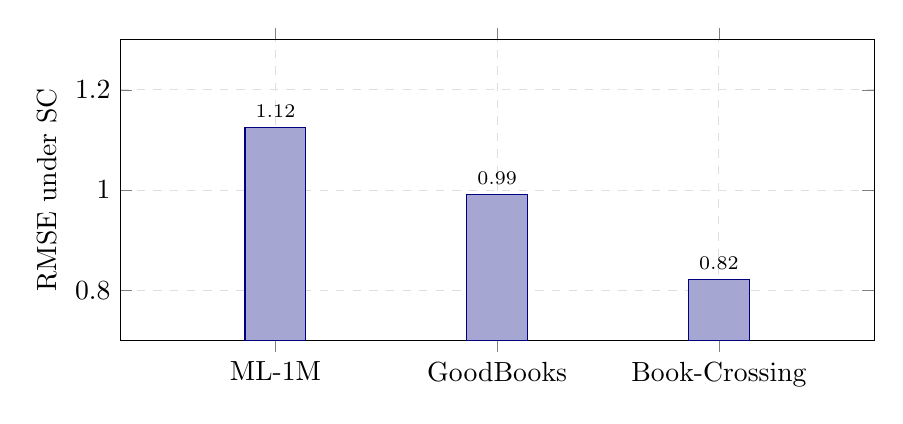
\begin{tikzpicture}
\begin{axis}[
    width=0.92\columnwidth, height=5.4cm,
    ybar, bar width=22pt,
    ylabel={RMSE under SC},
    symbolic x coords={ML-1M,GoodBooks,Book-Crossing},
    xtick=data,
    ymin=0.7, ymax=1.30,
    enlarge x limits=0.35,
    nodes near coords, nodes near coords style={font=\scriptsize},
    grid=major, grid style={dashed,gray!25},
]
\addplot[fill=blue!50!black!35, draw=blue!50!black] coordinates {
(ML-1M,1.1249) (GoodBooks,0.9916) (Book-Crossing,0.8214)};
\end{axis}
\end{tikzpicture}
\caption{Functional collapse under strict cold-start. UserBias produces RMSE \emph{identical} to GlobalMean on all three datasets ($\Delta$RMSE~$=0.00000$): the user-bias term is unestimable for unseen test users, so UserBias degenerates exactly to GlobalMean. The single bar per dataset represents both models.}
\label{fig:collapse}
\end{figure}

Consistent with Proposition~\ref{prop:collapse}, the user-specific bias term in UserBias has no training signal under SC and defaults to zero, so UserBias and GlobalMean yield identical predictions. The collapse propagates one level up: UserItemBias-SC collapses toward ItemBias-SC, with the residual user-bias contribution shrinking to differences of $0.00037$--$0.00493$ RMSE. These residuals are attributable to regularization rather than to a user-side signal.

\subsection{Protocol-Dependent Ranking Shifts Reach Ten Positions}
\label{sec:reversal}

\begin{figure}[!t]
\centering
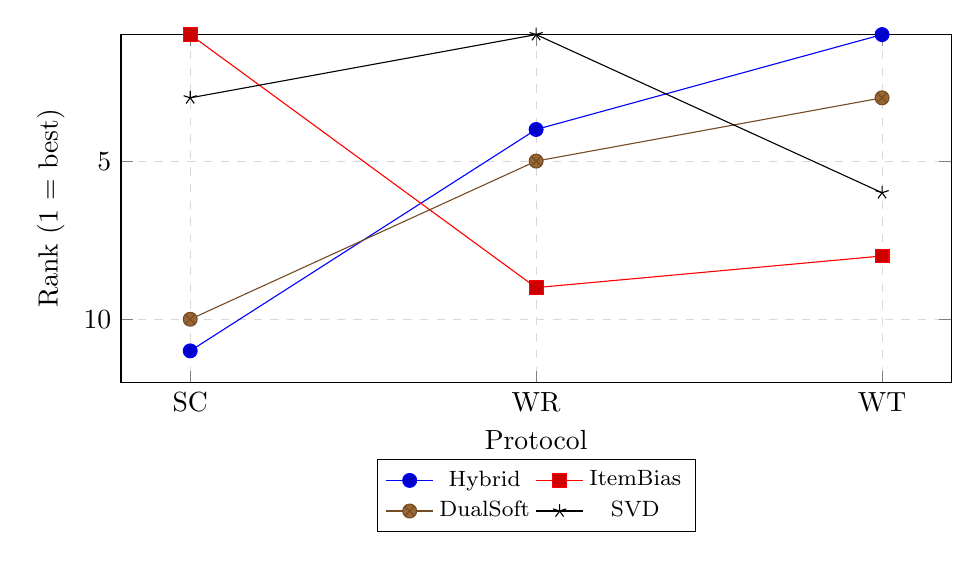
\begin{tikzpicture}
\begin{axis}[
    width=\columnwidth, height=6cm,
    xlabel={Protocol}, ylabel={Rank (1 = best)},
    symbolic x coords={SC,WR,WT},
    xtick=data,
    ymin=1, ymax=12,
    y dir=reverse,
    legend style={font=\footnotesize, at={(0.5,-0.22)}, anchor=north, legend columns=2},
    grid=major, grid style={dashed,gray!30},
    mark size=2.5pt,
]
\addplot coordinates {(SC,11) (WR,4) (WT,1)};
\addlegendentry{Hybrid}
\addplot coordinates {(SC,1) (WR,9) (WT,8)};
\addlegendentry{ItemBias}
\addplot coordinates {(SC,10) (WR,5) (WT,3)};
\addlegendentry{DualSoft}
\addplot coordinates {(SC,3) (WR,1) (WT,6)};
\addlegendentry{SVD}
\end{axis}
\end{tikzpicture}
\caption{Model rank across protocols on GoodBooks (3 seeds, lower is better). Hybrid rises from SC rank 11 to WT rank 1 (a 10-position shift), while ItemBias falls from SC rank 1 to WT rank 8: no model is universally best, and protocol choice determines the winner.}
\label{fig:reversal}
\end{figure}

Rank shifts are systematic rather than isolated to a single model. On GoodBooks, Hybrid rises from SC rank 11 to WT rank 1, a 10-position shift; on ML-1M, BehaviorMLP shifts by 8 positions (SC rank 11 to WT rank 3); and ItemBias shifts by 7 positions on ML-1M (SC rank 1 to WR rank 8). Across all 12 models, multiple models exhibit large protocol-conditional advantages. The conclusion is that there is no cross-protocol universal best model---the winner is selected by the protocol.

\subsection{Inter-Protocol Kendall $\tau$ Approaches Zero}
\label{sec:kendall_results}

\begin{table}[!t]
\centering
\caption{Inter-protocol Kendall $\tau$ on model rankings (12 models, 3 seeds). Lower $\tau$ means weaker consistency; GoodBooks SC-vs-WT is essentially uncorrelated.}
\label{tab:kendall}
\footnotesize
\begin{tabular}{@{}llc@{}}
\toprule
Dataset & Protocol pair & Kendall $\tau$ \\
\midrule
ML-1M         & SC vs.\ WR & 0.606 \\
ML-1M         & SC vs.\ WT & 0.303 \\
ML-1M         & WR vs.\ WT & 0.576 \\
GoodBooks     & SC vs.\ WR & 0.333 \\
GoodBooks     & SC vs.\ WT & \textbf{$-$0.030} \\
GoodBooks     & WR vs.\ WT & 0.455 \\
Book-Crossing & SC vs.\ WR & 0.576 \\
\bottomrule
\end{tabular}
\end{table}

Inter-protocol Kendall $\tau$ values are far below $1$. The most extreme case is GoodBooks SC-vs-WT with $\tau=-0.030$, i.e., the SC and WT rankings are essentially uncorrelated. Even the most consistent pair (ML-1M SC-vs-WR, $\tau=0.606$) leaves substantial rank disagreement. This quantifies the qualitative observation that different protocols effectively select different models.

\subsection{Protocol Regret Distinguishes Robust Models from Specialized Models}
\label{sec:regret_results}

\begin{table}[!t]
\centering
\caption{Protocol regret on ML-1M (3 seeds), sorted by mean regret. Mean regret averages over SC/WR/WT; worst regret is the maximum per-protocol regret.}
\label{tab:regret}
\footnotesize
\begin{tabular}{@{}lcc@{}}
\toprule
Model & Mean regret & Worst regret \\
\midrule
Hybrid        & 0.0098 & 0.0213 \\
SVD           & 0.0101 & 0.0281 \\
UserItemBias  & 0.0137 & 0.0302 \\
DualSoft      & 0.0330 & 0.0823 \\
ItemBias      & 0.0386 & 0.0769 \\
DualHard      & 0.0413 & 0.1026 \\
NeuMF         & 0.0593 & 0.1019 \\
BehaviorMLP   & 0.0976 & 0.2710 \\
ProfileMLP    & 0.1350 & 0.1612 \\
UserBias      & 0.1470 & 0.1699 \\
GlobalMean    & 0.1767 & 0.2119 \\
DeepFM        & 0.3459 & 0.3636 \\
\bottomrule
\end{tabular}
\end{table}

\begin{figure}[!t]
\centering
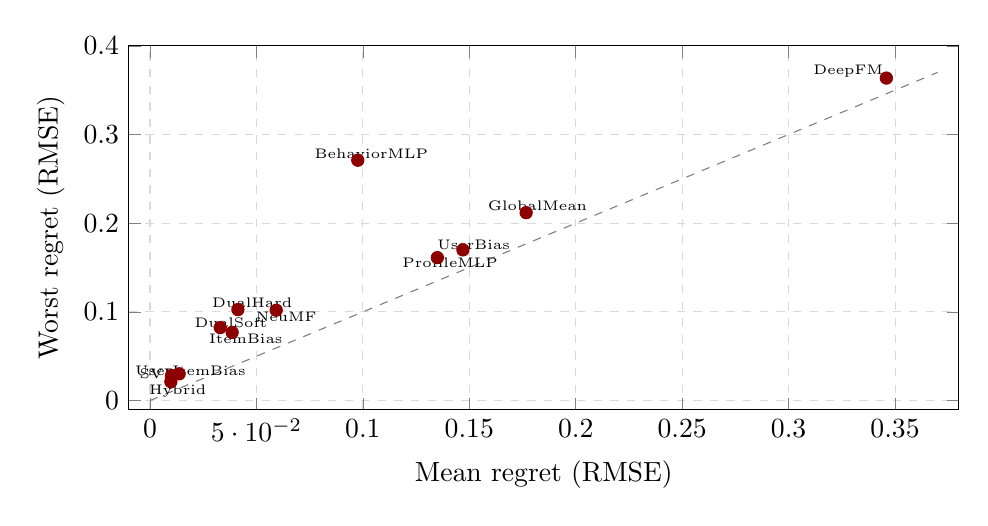
\begin{tikzpicture}
\begin{axis}[
    width=\columnwidth, height=6.2cm,
    xlabel={Mean regret (RMSE)}, ylabel={Worst regret (RMSE)},
    xmin=-0.01, xmax=0.38, ymin=-0.01, ymax=0.40,
    grid=major, grid style={dashed,gray!30},
    clip=false,
]
\draw[dashed, gray] (axis cs:0,0) -- (axis cs:0.37,0.37);
\addplot[only marks, mark=*, mark size=2.2pt, color=red!55!black] coordinates {
(0.1767,0.2119) (0.1470,0.1699) (0.0386,0.0769) (0.0137,0.0302)
(0.0101,0.0281) (0.0593,0.1019) (0.3459,0.3636) (0.0976,0.2710)
(0.1350,0.1612) (0.0098,0.0213) (0.0413,0.1026) (0.0330,0.0823)
};
\node[font=\tiny] at (axis cs:0.182,0.220) {GlobalMean};
\node[font=\tiny] at (axis cs:0.152,0.176) {UserBias};
\node[font=\tiny] at (axis cs:0.045,0.070) {ItemBias};
\node[font=\tiny] at (axis cs:0.019,0.034) {UserItemBias};
\node[font=\tiny] at (axis cs:0.004,0.030) {SVD};
\node[font=\tiny] at (axis cs:0.064,0.094) {NeuMF};
\node[font=\tiny] at (axis cs:0.328,0.372) {DeepFM};
\node[font=\tiny] at (axis cs:0.104,0.278) {BehaviorMLP};
\node[font=\tiny] at (axis cs:0.141,0.155) {ProfileMLP};
\node[font=\tiny] at (axis cs:0.013,0.011) {Hybrid};
\node[font=\tiny] at (axis cs:0.048,0.110) {DualHard};
\node[font=\tiny] at (axis cs:0.038,0.088) {DualSoft};
\end{axis}
\end{tikzpicture}
\caption{Mean vs.\ worst regret on ML-1M (3 seeds). The bottom-left cluster (Hybrid, SVD, UserItemBias) is robust; points far above the diagonal, especially BehaviorMLP (mean 0.098, worst 0.271), are protocol-specialized---good on average but with a large worst-case gap.}
\label{fig:regret}
\end{figure}

Regret separates robust from specialized models. On ML-1M, Hybrid, SVD, and UserItemBias form a robust cluster with mean regret $\leq 0.014$ and worst regret $\leq 0.030$. BehaviorMLP is the clearest specialized case: its mean regret (0.0976) is moderate but its worst regret (0.2710) is large, because it ranks 11th under SC (regret 0.2710) yet 3rd under WT (regret 0.0020). DeepFM is simply weak under all protocols (mean 0.3459, worst 0.3636). The mean/worst regret pair therefore exposes a trade-off that a single-protocol ranking hides.

\subsection{PSI Quantifies Per-Model Protocol Sensitivity}
\label{sec:psi_results}

\begin{table}[!t]
\centering
\caption{Protocol Sensitivity Index (PSI) by dataset (3 seeds). Higher PSI = stronger protocol dependence. Note: PSI is agnostic to absolute performance---a high PSI can reflect either a protocol-specialized strength or a protocol-conditional weakness, and a PSI of 0 can indicate uniform robustness or uniformly poor performance. PSI should therefore be read alongside Protocol Regret (Table~\ref{tab:regret}).}
\label{tab:psi}
\footnotesize
\begin{tabular}{@{}lccc@{}}
\toprule
Model & {ML-1M} & {GoodBooks} & {BC} \\
\midrule
GlobalMean    & 2 & 4  & 2 \\
UserBias      & 1 & 2  & 5 \\
ItemBias      & 7 & 8  & 4 \\
UserItemBias  & 4 & 3  & 1 \\
SVD           & 4 & 5  & 2 \\
NeuMF         & 3 & 4  & 1 \\
DeepFM        & 0 & 3  & 3 \\
BehaviorMLP   & 8 & 3  & 1 \\
ProfileMLP    & 2 & 4  & 3 \\
Hybrid        & 2 & \textbf{10} & 1 \\
DualHard      & 3 & 4  & 3 \\
DualSoft      & 5 & 7  & 0 \\
\bottomrule
\end{tabular}
\end{table}

Hybrid reaches PSI$=$10 on GoodBooks because it ranks 11th under SC but 1st under WT, the largest single-model shift in the study. BehaviorMLP reaches PSI$=$8 on ML-1M (SC rank 11 to WT rank 3). At the other extreme, DeepFM has PSI$=$0 on ML-1M because it ranks last under all three protocols---insensitivity here reflects consistent poor performance rather than robustness. PSI therefore needs to be read alongside absolute regret.

\subsection{Complexity Does Not Reliably Predict Robustness}
\label{sec:gap}

Within the warm-random protocol, each test sample is labeled as cold, medium, or warm based on the user's training-set activity. We define the Activity Gap as:
\begin{equation}
\mathrm{Gap}_m = \mathrm{RMSE}_{\mathrm{cold}} - \mathrm{RMSE}_{\mathrm{warm}}
\label{eq:gap}
\end{equation}

\begin{table}[!t]
\centering
\caption{Activity-segment RMSE gap on ML-1M warm-random (3 seeds). Gap = cold-segment RMSE $-$ warm-segment RMSE.}
\label{tab:gap}
\footnotesize
\begin{tabular}{@{}lcccc@{}}
\toprule
Model & {Cmplx.} & {Cold RMSE} & {Warm RMSE} & {Gap} \\
\midrule
DualHard      & 4 & 1.0981 & 0.9096 & \textbf{0.1884} \\
BehaviorMLP   & 3 & 1.0434 & 0.9119 & 0.1315 \\
Hybrid        & 3 & 1.0249 & 0.8994 & 0.1255 \\
NeuMF         & 3 & 1.0301 & 0.9066 & 0.1236 \\
DualSoft      & 4 & 1.0127 & 0.9093 & 0.1035 \\
DeepFM        & 3 & 1.3436 & 1.2439 & 0.0997 \\
SVD           & 2 & 0.9875 & 0.8918 & 0.0956 \\
UserItemBias  & 1 & 0.9840 & 0.9009 & 0.0830 \\
ItemBias      & 1 & 1.0389 & 0.9738 & 0.0651 \\
UserBias      & 1 & 1.0676 & 1.0281 & 0.0395 \\
ProfileMLP    & 3 & 1.0974 & 1.0598 & 0.0376 \\
GlobalMean    & 1 & 1.1446 & 1.1102 & 0.0344 \\
\bottomrule
\end{tabular}
\end{table}

\begin{figure}[!t]
\centering
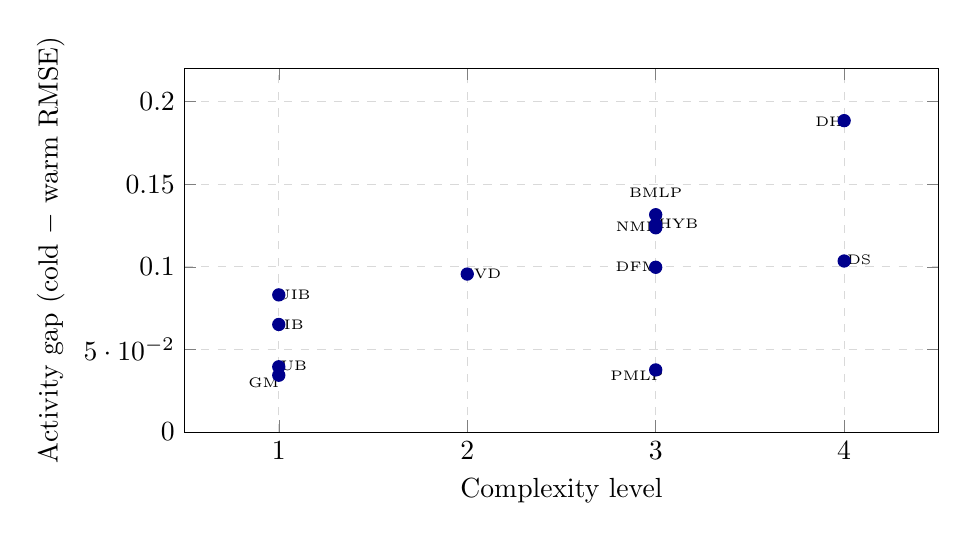
\begin{tikzpicture}
\begin{axis}[
    width=0.92\columnwidth, height=6.2cm,
    xlabel={Complexity level}, ylabel={Activity gap (cold $-$ warm RMSE)},
    xmin=0.5, xmax=4.5, xtick={1,2,3,4},
    ymin=0, ymax=0.22,
    grid=major, grid style={dashed,gray!30},
    clip=false,
]
\addplot[only marks, mark=*, mark size=2.2pt, color=blue!55!black] coordinates {
(1,0.0344) (1,0.0395) (1,0.0651) (1,0.0830)
(2,0.0956)
(3,0.0376) (3,0.0997) (3,0.1236) (3,0.1255) (3,0.1315)
(4,0.1035) (4,0.1884)
};
\node[font=\tiny] at (axis cs:0.92,0.030) {GM};
\node[font=\tiny] at (axis cs:1.08,0.040) {UB};
\node[font=\tiny] at (axis cs:1.08,0.065) {IB};
\node[font=\tiny] at (axis cs:1.08,0.083) {UIB};
\node[font=\tiny] at (axis cs:2.08,0.096) {SVD};
\node[font=\tiny] at (axis cs:2.9,0.034) {PMLP};
\node[font=\tiny] at (axis cs:2.9,0.100) {DFM};
\node[font=\tiny] at (axis cs:2.9,0.124) {NMF};
\node[font=\tiny] at (axis cs:3.12,0.126) {HYB};
\node[font=\tiny] at (axis cs:3.0,0.145) {BMLP};
\node[font=\tiny] at (axis cs:4.08,0.104) {DS};
\node[font=\tiny] at (axis cs:3.92,0.188) {DH};
\end{axis}
\end{tikzpicture}
\caption{Complexity vs.\ activity gap on ML-1M warm-random (3 seeds). Complexity weakly correlates with the gap; DualHard is largest, while complexity-3 models span the full range, refuting a simple complexity-to-robustness mapping.}
\label{fig:gap}
\end{figure}

A weak positive trend between complexity and the activity gap is visible: Bias models (complexity 1) cluster at gaps of $0.034$--$0.083$, while the largest gap belongs to DualHard (complexity 4, gap $0.1884$). However, the relationship is far from monotone---ProfileMLP (complexity 3) has the second-smallest gap ($0.0376$), and complexity-3 models span $0.038$--$0.132$. Model complexity therefore does not reliably predict robustness across user activity levels.

\subsection{Extreme Sparsity Favors Behavioral and Hybrid Models}
\label{sec:sparsity}

\begin{table}[!t]
\centering
\caption{Warm-random RMSE across datasets (3 seeds). Behavioral and hybrid models win under extreme sparsity (BC); SVD wins on denser datasets.}
\label{tab:sparsity}
\footnotesize
\begin{tabular}{@{}lccc@{}}
\toprule
Model & {BC (0.0015\%)} & {GB (0.73\%)} & {ML-1M (4.47\%)} \\
\midrule
GlobalMean    & 0.819 & 0.991 & 1.110 \\
UserBias      & 0.735 & 0.894 & 1.030 \\
ItemBias      & 0.807 & 0.953 & 0.975 \\
UserItemBias  & 0.724 & 0.854 & 0.906 \\
SVD           & 0.727 & \textbf{0.849} & \textbf{0.898} \\
NeuMF         & 0.749 & 0.855 & 0.916 \\
DeepFM        & 0.785 & 1.047 & 1.262 \\
BehaviorMLP   & 0.657 & 0.859 & 0.918 \\
ProfileMLP    & 0.811 & 0.979 & 1.060 \\
Hybrid        & \textbf{0.650} & 0.858 & 0.906 \\
DualHard      & 0.744 & 0.859 & 0.916 \\
DualSoft      & 0.675 & 0.859 & 0.915 \\
\bottomrule
\end{tabular}
\end{table}

\begin{figure*}[!t]
\centering
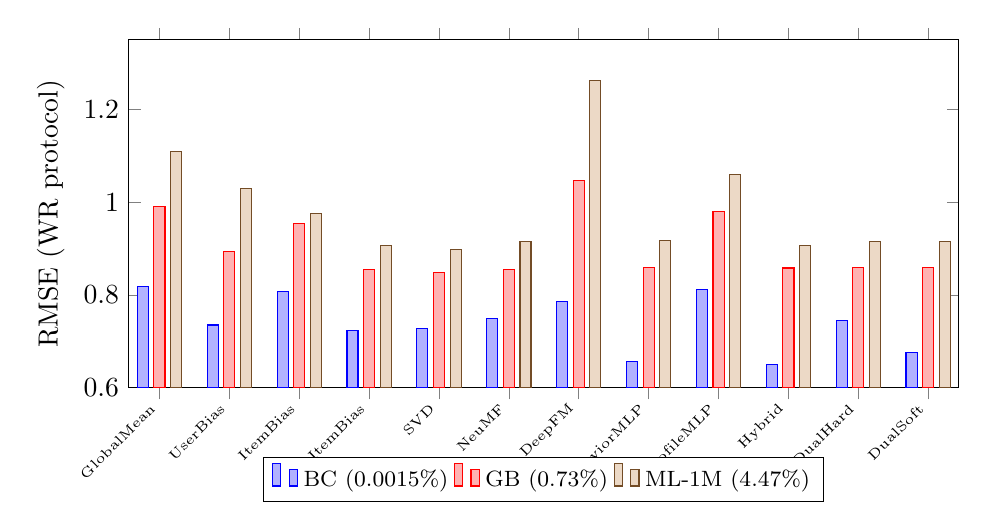
\begin{tikzpicture}
\begin{axis}[
    width=\textwidth, height=6cm,
    ybar, bar width=4pt,
    ylabel={RMSE (WR protocol)},
    symbolic x coords={GlobalMean,UserBias,ItemBias,UserItemBias,SVD,NeuMF,DeepFM,BehaviorMLP,ProfileMLP,Hybrid,DualHard,DualSoft},
    xtick=data, x tick label style={font=\tiny, rotate=45, anchor=east},
    legend style={font=\footnotesize, at={(0.5,-0.20)}, anchor=north, legend columns=3},
    ymin=0.6, ymax=1.35,
    enlarge x limits=0.04,
]
\addplot coordinates {(GlobalMean,0.819) (UserBias,0.735) (ItemBias,0.807) (UserItemBias,0.724) (SVD,0.727) (NeuMF,0.749) (DeepFM,0.785) (BehaviorMLP,0.657) (ProfileMLP,0.811) (Hybrid,0.650) (DualHard,0.744) (DualSoft,0.675)};
\addlegendentry{BC (0.0015\%)}
\addplot coordinates {(GlobalMean,0.991) (UserBias,0.894) (ItemBias,0.953) (UserItemBias,0.854) (SVD,0.849) (NeuMF,0.855) (DeepFM,1.047) (BehaviorMLP,0.859) (ProfileMLP,0.979) (Hybrid,0.858) (DualHard,0.859) (DualSoft,0.859)};
\addlegendentry{GB (0.73\%)}
\addplot coordinates {(GlobalMean,1.110) (UserBias,1.030) (ItemBias,0.975) (UserItemBias,0.906) (SVD,0.898) (NeuMF,0.916) (DeepFM,1.262) (BehaviorMLP,0.918) (ProfileMLP,1.060) (Hybrid,0.906) (DualHard,0.916) (DualSoft,0.915)};
\addlegendentry{ML-1M (4.47\%)}
\end{axis}
\end{tikzpicture}
\caption{Warm-random RMSE of all 12 models across the three datasets (3 seeds). Under extreme sparsity (BC), behavioral and hybrid models (BehaviorMLP, Hybrid, DualSoft) outperform all bias and MF baselines; on denser datasets (GB, ML-1M), SVD is best and the advantage of behavioral models disappears.}
\label{fig:sparsity}
\end{figure*}

The warm-random results reveal that models respond very differently to sparsity. Under extreme sparsity (Book-Crossing, $0.0015\%$ density), the behavioral and hybrid models---BehaviorMLP (0.657), Hybrid (0.650), and DualSoft (0.675)---outperform all bias and matrix-factorization baselines, indicating that profile/behavior features provide critical complementary signal when interactions are sparse. On the denser ML-1M and GoodBooks, SVD is best and these behavioral models lose their advantage. Sparsity thus interacts with model family: the relative effectiveness of behavioral fusion grows as density falls.

\subsection{Neural Modeling Pays Off Only Under Sparse Regimes}
\label{sec:bnr_results}

\begin{table}[!t]
\centering
\caption{Bias-Normalized RMSE (BNR) under warm-random (3 seeds). BNR $=$ RMSE$_m$/RMSE$_{best\_bias}$; values $<1.0$ (bold) indicate improvement over the best bias baseline.}
\label{tab:bnr}
\footnotesize
\begin{tabular}{@{}lccc@{}}
\toprule
Model & {ML-1M} & {GoodBooks} & {BC} \\
\midrule
GlobalMean    & 1.23 & 1.16 & 1.13 \\
UserBias      & 1.14 & 1.05 & 1.02 \\
ItemBias      & 1.08 & 1.12 & 1.12 \\
UserItemBias  & 1.00 & 1.00 & 1.00 \\
SVD           & \textbf{0.99} & 1.00 & 1.00 \\
NeuMF         & 1.01 & 1.00 & 1.03 \\
DeepFM        & 1.39 & 1.23 & 1.09 \\
BehaviorMLP   & 1.01 & 1.01 & \textbf{0.91} \\
ProfileMLP    & 1.17 & 1.15 & 1.12 \\
Hybrid        & 1.00 & 1.00 & \textbf{0.90} \\
DualHard      & 1.01 & 1.01 & 1.03 \\
DualSoft      & 1.01 & 1.01 & \textbf{0.93} \\
\bottomrule
\end{tabular}
\end{table}

\begin{figure}[!t]
\centering
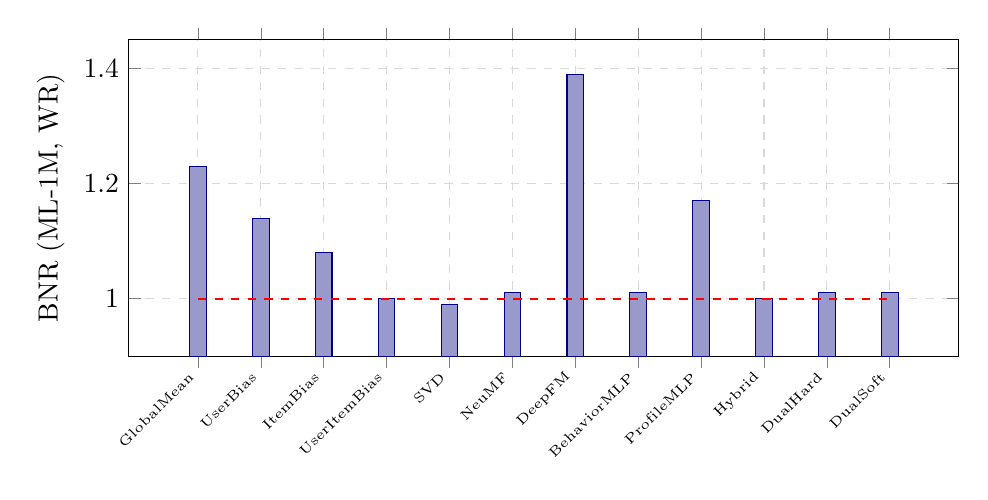
\begin{tikzpicture}
\begin{axis}[
    width=\columnwidth, height=5.6cm,
    ybar, bar width=6pt,
    ylabel={BNR (ML-1M, WR)},
    symbolic x coords={GlobalMean,UserBias,ItemBias,UserItemBias,SVD,NeuMF,DeepFM,BehaviorMLP,ProfileMLP,Hybrid,DualHard,DualSoft},
    xtick=data, x tick label style={font=\tiny, rotate=45, anchor=east},
    ymin=0.90, ymax=1.45,
    grid=major, grid style={dashed,gray!30},
]
\addplot[fill=blue!50!black!40, draw=blue!50!black] coordinates {
(GlobalMean,1.23) (UserBias,1.14) (ItemBias,1.08) (UserItemBias,1.00)
(SVD,0.99) (NeuMF,1.01) (DeepFM,1.39) (BehaviorMLP,1.01)
(ProfileMLP,1.17) (Hybrid,1.00) (DualHard,1.01) (DualSoft,1.01)};
\draw[dashed, red, thick] (axis cs:GlobalMean,1.0) -- (axis cs:DualSoft,1.0);
\end{axis}
\end{tikzpicture}
\caption{BNR on ML-1M under warm-random (3 seeds). The dashed line at BNR$=$1.0 is parity with the best bias baseline. Most neural and adaptive models sit within $\pm1\%$ of parity; only SVD marginally beats the baseline, while DeepFM is $39\%$ worse.}
\label{fig:bnr}
\end{figure}

On ML-1M and GoodBooks, most deep and adaptive models achieve BNR of $0.99$--$1.01$, i.e., within $\pm1\%$ of the best bias baseline, and only SVD marginally beats it (BNR$=$0.99 on ML-1M). The picture changes sharply under extreme sparsity: on Book-Crossing, BehaviorMLP (0.91), Hybrid (0.90), and DualSoft (0.93) reach BNR well below 1.0, a $7$--$10\%$ RMSE reduction over the best bias baseline. BNR thus confirms that the value of neural/behavioral modeling over bias baselines is protocol- and sparsity-dependent, not universal.

\subsection{End-to-End Gating Yields Inconsistent Gains}
\label{sec:e2e}

As a supplementary analysis, we compare end-to-end trained gating with the two-stage training strategy for DualSoftGating. The values below are from a representative single run (seed 2024); the multi-seed main results for DualSoft are reported in Table~\ref{tab:main_results}.

\begin{table}[!t]
\centering
\caption{E2E vs.\ two-stage gating (DualSoftGating RMSE, representative run seed 2024). E2E helps only on ML-1M strict cold-start; gains elsewhere are negligible or negative.}
\label{tab:e2e}
\footnotesize
\begin{tabular}{@{}llccc@{}}
\toprule
Dataset & {Protocol} & {2-Stage} & {E2E} & {$\Delta$} \\
\midrule
ML-1M & SC & 1.0883 & \textbf{1.0220} & $-$0.0663 \\
ML-1M & WR & 0.9148 & 0.9117          & $-$0.0030 \\
ML-1M & WT & 0.9238 & 0.9237          & $-$0.0001 \\
GB    & SC & 1.0063 & 1.1550          & +0.1487  \\
GB    & WR & 0.8592 & 0.8592          & 0.0000   \\
GB    & WT & 0.8607 & 0.8603          & $-$0.0004 \\
\bottomrule
\end{tabular}
\end{table}

E2E gating provides limited and inconsistent improvements. Although it improves performance on ML-1M strict cold-start (0.066 RMSE reduction), the gains on warm protocols are negligible ($<0.003$). On GoodBooks strict cold-start, E2E actually degrades performance by 0.149. We therefore report E2E gating as an auxiliary analysis rather than a central contribution.

\subsection{Ranking-Metric Validation}
\label{sec:ranking_validation}

Because recommender-system research often emphasizes ranking quality, we additionally report NDCG@10 computed from the same predictions and averaged over the three seeds. Recall@10 is omitted because rating-prediction test sets contain few items per user, making per-user Recall@10 numerically near zero ($<\!0.0002$) and uninformative; this is a known limitation of evaluating rating-prediction models with top-$N$ metrics.

\begin{table}[!t]
\centering
\caption{NDCG@10 (mean over 3 seeds). Best per column in bold. The collapse pattern is preserved: under SC, UserBias again equals GlobalMean on all three datasets.}
\label{tab:ndcg}
\footnotesize
\begin{tabular}{@{}lcccccc@{}}
\toprule
& \multicolumn{2}{c}{ML-1M} & \multicolumn{2}{c}{GoodBooks} & \multicolumn{2}{c}{Book-Crossing} \\
\cmidrule(lr){2-3}\cmidrule(lr){4-5}\cmidrule(lr){6-7}
Model & SC & WR & SC & WR & SC & WR \\
\midrule
GlobalMean    & 0.874 & 0.287 & 0.881 & 0.703 & 0.467 & 0.699 \\
UserBias      & 0.874 & 0.927 & 0.881 & \textbf{1.000} & 0.467 & \textbf{1.000} \\
ItemBias      & 0.935 & 0.886 & \textbf{1.000} & 0.978 & 0.909 & 0.880 \\
UserItemBias  & 0.863 & 0.932 & 0.894 & \textbf{1.000} & 0.963 & 0.947 \\
SVD           & 0.918 & \textbf{1.000} & 0.830 & 0.954 & 0.954 & 0.940 \\
NeuMF         & 0.894 & 0.955 & 0.954 & \textbf{1.000} & 0.963 & 0.898 \\
DeepFM        & \textbf{0.949} & 0.885 & \textbf{1.000} & \textbf{1.000} & 0.741 & 0.899 \\
BehaviorMLP   & 0.696 & \textbf{1.000} & 0.804 & \textbf{1.000} & 0.954 & \textbf{1.000} \\
ProfileMLP    & 0.946 & 0.927 & 0.979 & 0.968 & 0.934 & 0.927 \\
Hybrid        & 0.693 & 0.954 & 0.721 & \textbf{1.000} & 0.953 & \textbf{1.000} \\
DualHard      & 0.932 & 0.927 & 0.949 & \textbf{1.000} & \textbf{1.000} & 0.963 \\
DualSoft      & 0.694 & \textbf{1.000} & 0.726 & \textbf{1.000} & 0.934 & 0.898 \\
\bottomrule
\end{tabular}
\end{table}

Two observations follow. First, the functional collapse is preserved under NDCG@10: UserBias again equals GlobalMean exactly on SC across all three datasets (0.874/0.881/0.467), confirming that the collapse is metric-independent and reflects a change in the effective model rather than a peculiarity of RMSE. Second, the protocol preference structure is broadly consistent with the RMSE-based findings---SC favors item-side priors (ItemBias, DeepFM), while WR favors models with estimable user parameters (UserBias, SVD, Hybrid)---although NDCG@10 saturates near 1.0 under WR for several models, reflecting the low candidate counts per user in rating-prediction test sets. The ranking-metric analysis therefore corroborates rather than overturns the RMSE-based conclusions.

\FloatBarrier

% ============================================================================
% 5. DISCUSSION
% ============================================================================
\section{Discussion}
\label{sec:discussion}

\subsection{Protocol-Induced Functional Collapse: A Mechanism}
As formalized in Section~\ref{sec:formal_collapse}, functional collapse is a property of the estimable parameter set: under SC, the per-user term $b_u$ is unestimable for any test user, so UserBias and UserItemBias reduce to their simpler submodels (GlobalMean and ItemBias respectively). The empirical results in Table~\ref{tab:collapse} confirm this exactly ($\Delta$RMSE~$=0.00000$). The practical implication is that the loss is silent---it appears only when one inspects which terms are functionally active. A practitioner who deploys UserBias under SC is, in effect, deploying GlobalMean, and this mechanism generalizes to any model component whose parameters depend on entities absent from the training split.

\subsection{Protocol Preference Structure}
The three protocols favor structurally different signals, which directly informs how a practitioner should match a model to a deployment scenario:
\begin{itemize}
    \item For \emph{new-user onboarding} (SC), item-side priors are safer than user-specific parameters because user-level signals are unavailable at test time; accordingly ItemBias and SVD win on ML-1M and GoodBooks (ItemBias rank 1, SVD rank 2--3), because item statistics and latent item factors remain estimable.
    \item For \emph{existing-user recommendation under random splits} (WR), collaborative models remain competitive because user-specific parameters are estimable; the same user appears in train and test, so SVD/UserItemBias dominate (SVD rank 1 on ML-1M and GoodBooks).
    \item For \emph{temporally shifted environments} (WT), behavioral and adaptive models become more attractive because static user factors may become stale; models that fuse behavior/profile signals or adaptively route between cold and warm regimes win (DualSoft rank 1 on ML-1M; Hybrid rank 1 on GoodBooks).
\end{itemize}
This family $\times$ protocol interaction is systematic, not noise: it reproduces across three seeds and three datasets, and is reflected both in the per-protocol winners and in the near-zero Kendall $\tau$ (GoodBooks SC-vs-WT $= -0.030$).

\subsection{Specialized vs.\ Robust Models: The Regret Trade-off}
Protocol Regret separates models that are robust from those that are specialized. The robust cluster (Hybrid, SVD, UserItemBias on ML-1M) has low mean \emph{and} low worst regret; these models are safe default choices. Specialized models such as BehaviorMLP have moderate mean regret but large worst regret (0.271 on ML-1M): they are excellent on their favored protocol (WT regret 0.002) but poor elsewhere (SC regret 0.271). A practitioner optimizing for a single known protocol should pick the specialized winner; one facing an unknown or mixed deployment should prefer the robust cluster. Crucially, this trade-off is invisible to a single-protocol ranking and only surfaces when mean and worst regret are reported together.

\subsection{BNR: When Neural Modeling Pays Off}
BNR shows that on ML-1M and GoodBooks, most neural and adaptive models are within $\pm1\%$ of the best bias baseline, and only SVD marginally beats it. The computational overhead of deep models is not justified for rating prediction on these datasets under WR. The exception is extreme sparsity: on Book-Crossing, behavioral and adaptive models (BehaviorMLP, Hybrid, DualSoft) reach BNR 0.90--0.93, a 7--10\% RMSE reduction over the best bias baseline. BNR thus localizes the value of neural/behavioral modeling to sparse regimes rather than treating complexity as universally beneficial.

\subsection{Practical Implications}
Our findings yield directly actionable guidelines for practitioners facing protocol-aware model selection:
\begin{itemize}
    \item \textbf{Cold-start deployment (new-user onboarding).} Prioritize ItemBias or SVD; avoid UserBias, which functionally collapses to GlobalMean under SC and provides no user-side signal.
    \item \textbf{Warm-random split (standard offline A/B test).} SVD and UserItemBias offer the best robustness--accuracy trade-off; most deep models add $<$1\% over the best bias baseline and are not cost-justified on dense data.
    \item \textbf{Warm-temporal split (time-drifted environments).} Hybrid or DualSoft are preferred, as static collaborative signals become stale and behavioral/fused/adaptive models better track temporal drift.
    \item \textbf{Extreme sparsity ($<$0.01\% density).} Behavioral fusion models (BehaviorMLP, Hybrid) outperform traditional matrix factorization, yielding a 7--10\% RMSE reduction over the best bias baseline; profile-only models (ProfileMLP) do not suffice.
    \item \textbf{Unknown or mixed deployment.} Prefer the robust cluster identified by low mean \emph{and} low worst Protocol Regret (e.g., Hybrid, SVD, UserItemBias on ML-1M) over specialized winners that collapse outside their favored protocol.
\end{itemize}

% ============================================================================
% 6. CONCLUSION
% ============================================================================
\FloatBarrier
\section{Conclusion}
\label{sec:conclusion}

This paper presented a controlled multi-seed empirical study of how evaluation protocols change the effective model in rating-prediction recommender systems. Across 12 models, three datasets, eight dataset--protocol combinations, and three seeds (288 runs), we found:

\begin{enumerate}
    \item \textbf{Multi-protocol, multi-seed unified evaluation.} Protocols systematically reorder model rankings, with rank shifts up to 10 positions and inter-protocol Kendall $\tau$ as low as $-0.030$ (GoodBooks SC-vs-WT); no model is universally best.
    \item \textbf{Protocol-induced functional collapse.} Under strict cold-start, UserBias degenerates exactly to GlobalMean (diff$=$0.00000) and UserItemBias collapses toward ItemBias, because user-specific terms are unestimable for unseen test users. The protocol silently rewrites the effective model.
    \item \textbf{Model-family $\times$ protocol systematic interaction.} SC favors item-bias and matrix factorization, WR favors static collaborative models, and WT favors behavioral, fused, and adaptive models---a pattern that reproduces across seeds and datasets.
    \item \textbf{A protocol-robustness evaluation framework.} PSI, inter-protocol Kendall $\tau$, and Protocol Regret jointly expose protocol sensitivity, ranking inconsistency, and the specialized-vs-robust trade-off that single-protocol rankings hide.
\end{enumerate}

These findings suggest that recommender-system evaluation should report results across multiple protocols and seeds, and adopt protocol-robustness diagnostics rather than relying on a single-protocol point estimate. The findings are established for explicit rating prediction and should not be directly assumed to hold for top-$N$ recommendation, implicit feedback, or session-based recommendation without further validation.

\FloatBarrier
\section{Limitations}
\label{sec:limitations}

We acknowledge several boundaries of this study, each of which also points to a promising direction for future work:

\begin{enumerate}
    \item \textbf{Reproducibility scope.} Following common practice in multi-seed recommender-system evaluation, we report mean and standard deviation over three independent random seeds (2024/2025/2026) to ensure reproducibility. We focus on effect sizes (mean $\pm$ std, rank shifts, Kendall $\tau$, regret) rather than $p$-values; extending the framework to larger-scale statistical testing and user-level bootstrap confidence intervals is a natural next step.
    \item \textbf{Rating-prediction task.} We focus on rating-prediction protocols; extending the diagnostic framework to top-$N$ recommendation and ranking metrics is a promising direction.
    \item \textbf{Book-Crossing has no timestamps.} The Book-Crossing dataset lacks timestamp information, so only SC and WR are evaluated on it; the WT protocol is unavailable for this dataset.
    \item \textbf{Model scope.} This study covers Bias, MF, Deep, and Adaptive families. Graph-based recommenders such as NGCF~\cite{wang2019ngcf} and LightGCN~\cite{he2020lightgcn} are not included in the current scope; their protocol sensitivity---particularly how user-node embeddings behave under strict cold-start, where test users have no edges in the training graph---warrants separate investigation as a promising future direction.
    \item \textbf{Cost accounting.} We do not record parameter counts or training time. BNR reflects relative RMSE against a bias baseline rather than computational cost-effectiveness; a full cost--benefit analysis that incorporates parameter count, training time, and inference latency is left to future work.
\end{enumerate}

\begin{thebibliography}{00}

\bibitem{schafer2007collaborative}
J. Schafer, D. Frankowski, J. Herlocker, and S. Sen, ``Collaborative filtering recommender systems,'' in \textit{The Adaptive Web}, Springer, 2007, pp. 291--324.

\bibitem{koren2009matrix}
Y. Koren, R. Bell, and C. Volinsky, ``Matrix factorization techniques for recommender systems,'' \textit{Computer}, vol. 42, no. 8, pp. 30--37, 2009.

\bibitem{bell2007bellkor}
R. M. Bell, Y. Koren, and C. Volinsky, ``The BellKor solution to the Netflix Grand Prize,'' \textit{Netflix Prize Documentation}, 2009.

\bibitem{he2017neural}
X. He, L. Liao, H. Zhang, L. Nie, X. Hu, and T.-S. Chua, ``Neural collaborative filtering,'' in \textit{Proc. WWW}, 2017, pp. 173--182.

\bibitem{guo2017deepfm}
H. Guo, R. Tang, Y. Ye, Z. Li, and X. He, ``DeepFM: A factorization-machine based neural network for CTR prediction,'' in \textit{Proc. IJCAI}, 2017, pp. 1725--1731.

\bibitem{schein2002methods}
A. I. Schein, A. Popescul, L. H. Ungar, and D. M. Pennock, ``Methods and metrics for cold-start recommendations,'' in \textit{Proc. SIGIR}, 2002, pp. 253--260.

\bibitem{vartak2017meta}
M. Vartak, A. Thiagarajan, C. Wang, J. Helmke, and J. B. Pineau, ``A meta-learning approach for cold-start recommendation,'' in \textit{Proc. AISTATS}, 2017, pp. 1--10.

\bibitem{elkahky2015multi}
A. M. Elkahky, Y. Song, and X. He, ``A multi-view deep learning approach for cross domain user modeling in recommendation systems,'' in \textit{Proc. WWW}, 2015, pp. 278--288.

\bibitem{dacrema2019we}
M. F. Dacrema, P. Cremonesi, and D. Jannach, ``Are we really making much progress? A worrying analysis of recent neural recommendation approaches,'' in \textit{Proc. RecSys}, 2019, pp. 101--109.

\bibitem{rendle2009bpr}
S. Rendle, C. Freudenthaler, Z. Gantner, and L. Schmidt-Thieme, ``BPR: Bayesian personalized ranking from implicit feedback,'' in \textit{Proc. UAI}, 2009, pp. 452--461.

\bibitem{wang2019ngcf}
X. Wang, X. He, M. Wang, F. Feng, and T.-S. Chua, ``Neural graph collaborative filtering,'' in \textit{Proc. SIGIR}, 2019, pp. 165--174.

\bibitem{he2020lightgcn}
X. He, K. Deng, X. Wang, Y. Li, Y. Zhang, and M. Wang, ``LightGCN: Simplifying and powering graph convolution network for recommendation,'' in \textit{Proc. SIGIR}, 2020, pp. 639--648.

\bibitem{kang2018sasrec}
W.-C. Kang and J. McAuley, ``Self-attentive sequential recommendation,'' in \textit{Proc. ICDM}, 2018, pp. 197--206.

\bibitem{sun2019bert4rec}
F. Sun, J. Liu, J. Wu, J. Pei, X. Lin, W. Ou, and P. Jiang, ``BERT4Rec: Sequential recommendation with bidirectional encoder representations from transformer,'' in \textit{Proc. CIKM}, 2019, pp. 1441--1450.

\bibitem{dacrema2021troubling}
M. F. Dacrema, P. Cremonesi, and D. Jannach, ``A troubling analysis of reproducibility and progress in recommender systems research,'' \textit{ACM Trans. Inf. Syst.}, vol. 39, no. 2, pp. 1--49, 2021.

\bibitem{canamares2018should}
R. Ca{\~n}amares and P. Castells, ``Should I follow the crowd? A probabilistic analysis of the effectiveness of popularity in recommender systems,'' in \textit{Proc. SIGIR}, 2018, pp. 415--424.

\bibitem{steck2019ease}
S. Steck, ``Embarrassingly shallow autoencoders for sparse data,'' in \textit{Proc. WWW}, 2019, pp. 3251--3257.

\bibitem{gunawardana2009survey}
A. Gunawardana and G. Shani, ``A survey of accuracy evaluation metrics of recommendation tasks,'' \textit{J. Mach. Learn. Res.}, vol. 10, pp. 2935--2962, 2009.

\bibitem{covington2016deep}
P. Covington, J. Adams, and E. Sargin, ``Deep neural networks for YouTube recommendations,'' in \textit{Proc. RecSys}, 2016, pp. 191--198.

\bibitem{zhao2021recbole}
Y. Zhao, J. Xia, L. Jiang, et al., ``RecBole: Towards a unified, comprehensive and efficient framework for recommendation algorithms,'' in \textit{Proc. CIKM}, 2021, pp. 4653--4664.

\end{thebibliography}

\end{document}
